% !TEX root = ../../thesis.tex

\section{Intertext Clients} \label{intertextClients}

Intertext clients are the user facing products of Intertext, that builds the bridge between the user and servers that serve IUIDL. They are meant to be implemented natively for the host platform in the most optimal way possible. 

For example, on mobile platforms such as iOS and Andriod, UI elements would be larger and more suitable for touch interactions. Primary interaction would be translated as "tap" while secondary interactions, if any, would be translated as "tap and hold". The layout would adjust itself based on the screen size. The client would be implemented with either native technologies such as Swift/Objective-C for iOS and Kotlin/Java for Android, or with hybrid technologies that gets compiled into native code, such as React Native or Flutter for maximum responsiveness and efficiency. 

At the time of this paper, a web client and a command-line client is implemented. Native clients for iOS and Android, and desktop clients for Mac OS, Windows and several Linux distributions are among the ones that are planned, more could be found in \nameref{futureWork} section.

Intertext clients consists of two main parts; components and commands. Each Intertext client implement these separately, based on the host platform and its capabilities. Each client also implements the  their own local storage, state management strategy, and communication technique with the server.

\subsection{Components}

Components are anything that has a visual representation. All component stem from a generic IUIDL definition, and is interpreted based on the host platform requirements. They can be organisational or presentational. Organisational components are the layout components, they are used to position presentational components on the screen. Intertext implements a version of css flexbox specification as a layout system, which could be used to implement responsive interfaces for all screen sizes. For non-browser based platforms, we use the popular Yoga layout engine, which is a standalone implementation of the css flexbox specification in C++, allowing us to target almost any platform. More details on the layout system is given in \nameref{implementation} section.

Most presentational Intertext components share a concept, "intent", which is a way to communicate the intention of the UI element based on its use-case. Intertext clients renders the UI elements differently based on its intent, allowing a way for the developer to convey an intention of an UI element to the user without being able to intercept with the styles. For instance, an error message could be shown in a block component that has the intent "error", and it will be rendered with a red background, indicating to the user that it is an error message. \ref{fig:intents} shows an example of intents on block component for Intertext web client.

\begin{figure}
  \centering
  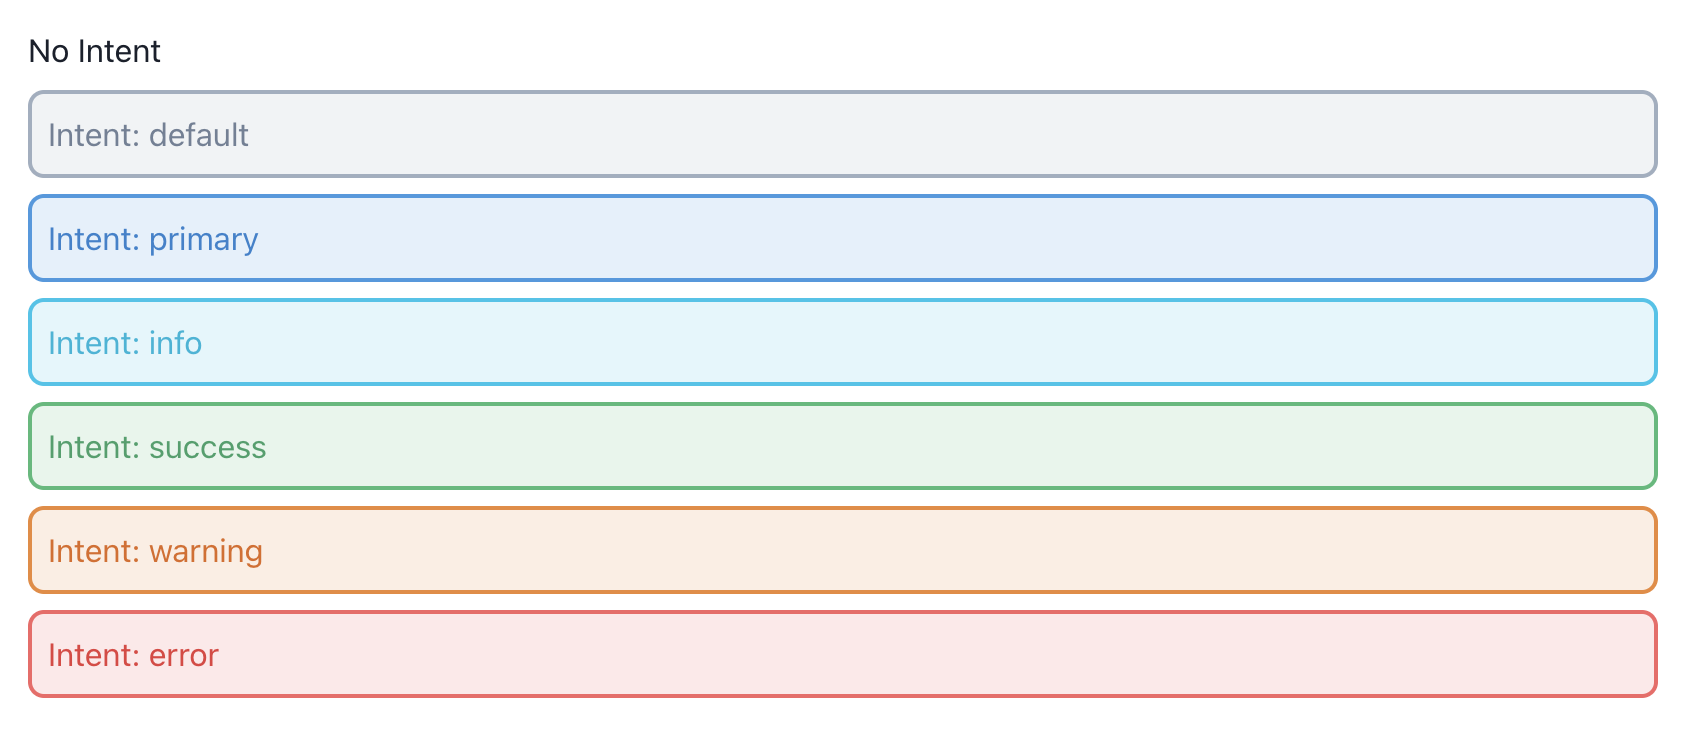
\includegraphics[width=13cm]{thesis/paper/images/intents.png}
  \caption{Intents for Block components}%
  \label{fig:intents}%
\end{figure}

\subsection{Commands}

Commands are IUIDL statements that are used to instruct Intertext client to take an action. These actions can be triggered upon interaction with some components (such as clicking a button or submitting a form), a life-cycle event or with a timeout. Commands are very primitive by design, they are not meant to build application logic with. They are merely for asking the Intertext client to communicate with the server, store something, read something that is stored, or retrieve some data from the user. Command system is designed in order to ensure Intertext client is aware of what it is being asked to do, so that it can control and restrict the entire flow, ask for permission from the user when necessary, or simply refuse to take an action and bail if needed. 

Figure \ref{fig:ex_cmd_post_timeout} shows an example of how a network request action can be executed upon a delay, and Figure \ref{fig:ex_cmd_form} how a form can be submitted with reference to input fields on the server side. More on commands are on \nameref{implementation} section.

\begin{figure}
\begin{minipage}{\linewidth}
\begin{lstlisting}[language=xml]
<timeout delay="1000">
  <post endpoint="/refresh"></post>
</timeout>
\end{lstlisting}
\end{minipage}
\caption{Post command on Timeout}%
\label{fig:ex_cmd_post_timeout}%
\end{figure}

\begin{figure}
\begin{minipage}{\linewidth}
\begin{lstlisting}[language=xml]
<form endpoint="/todo/save">
  <input name="item_title"></input>
  <input name="item_description"></input>
  <button>Submit</button>
</form>
\end{lstlisting}
\end{minipage}
\caption{Form command with reference on server side to internal input values}%
\label{fig:ex_cmd_form}%
\end{figure}

\subsection{State Management}

\subsection{Communication}



\begin{figure}
\begin{minipage}{\linewidth}
\begin{lstlisting}[language=xml]
<state key="current_page">4</state>
<button>
  Previous Page
  <button.onClick>
    <post endpoint="/items/previous_page"></post>
  </button.onClick>
</button>
<button>
  Next Page
  <button.onClick>
    <post endpoint="/items/next_page"></post>
  </button.onClick>
</button>
\end{lstlisting}
\end{minipage}
\caption{Setting state from server side}%
\label{fig:ex_cmd_post_state}%
\end{figure}

% - clients
%   - server-side rendering
%   - state
%   - layout
%   - communication
%     - ui manipulation technique
%       - front-end manipulation
%       - backend manipulation
%     - front-end state management


- Components
- Commands